\section{Implementacja}
\subsection{Interfejs użytkownika}
\label{GUI}
Zgodnie z założeniami projektu zbudowano aplikację w środowisku MATLAB umożliwiającą użytkownikowi szybkie przesyłanie danych do mikrokontrolera. Zadbano o intuicyjność graficznego interfejsu użytkownika udostępniając następujące funkcjonalności:
\begin{enumerate}
	
	\item Ręczne wprowadzanie kolejnych punktów charakterystyki.
	\item Automatyczne wprowadzanie częstotliwości po kliknięciu użytkownika na wykres.
	\item Wykres amplitudy oraz przesunięcia fazowego dla wprowadzonych punktów charakterystyki częstotliwościowej.
	\item Algorytm liczący sygnał w dziedzinie czasu na podstawie wprowadzonych przez użytkownika punktów (zgodnie z równaniem \ref{eq:alg}).
	\item Rysowanie odpowiedzi w dziedzinie czasu \textit{online}.
	\item Automatyczne skalowanie wykresów (skala liniowa, logarytmiczna).
	\item Możliwość wysłania wprowadzonej charakterystyki do mikrokontrolera (zgodnie z zaimplementowanym protokołem opisanym w podrozdziale \ref{PK}).
\end{enumerate} 
Po wprowadzeniu dwóch próbek aplikacja prezentuje się następująco:
\begin{figure}[h!]
	\centering
	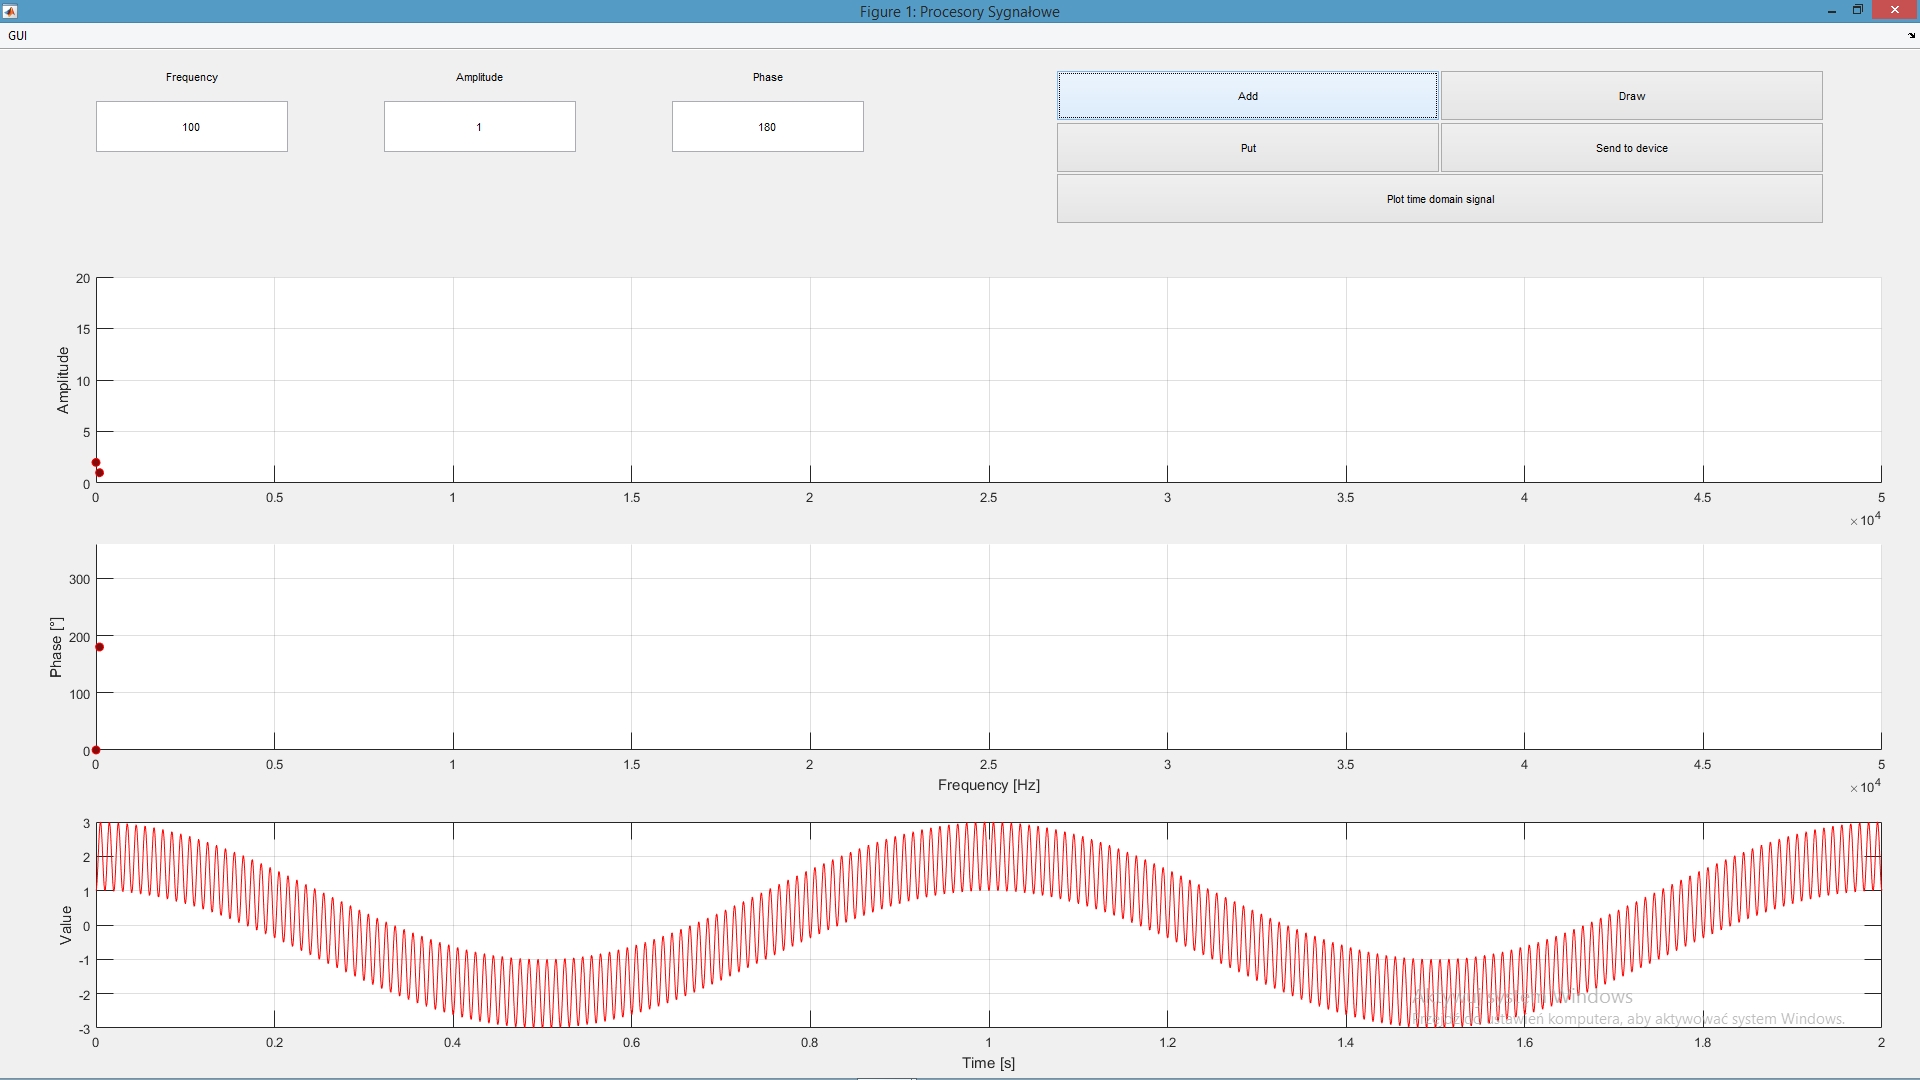
\includegraphics[scale = 0.3]{fig/GUI2.png}
	\caption		
	{Widok aplikacji po wprowadzeniu dwóch punktów na charakterystyce częstotliwościowej.}
	\label{gui1}
\end{figure}
Zakres wyświetlanych częstotliwości zgodny jest z założeniem opisanym równaniem \ref{eq:twP}. Po kliknięciu w zakładkę \textit{GUI} w menu użytkownik może wybrać jedną z opcji skalowania wykresów, a także zresetować aktualnie wprowadzone punkty lub zakończyć działanie aplikacji w sposób zapewniający zwolnienie wszystkich jej zasobów.
\begin{figure}[h!]
	\centering
	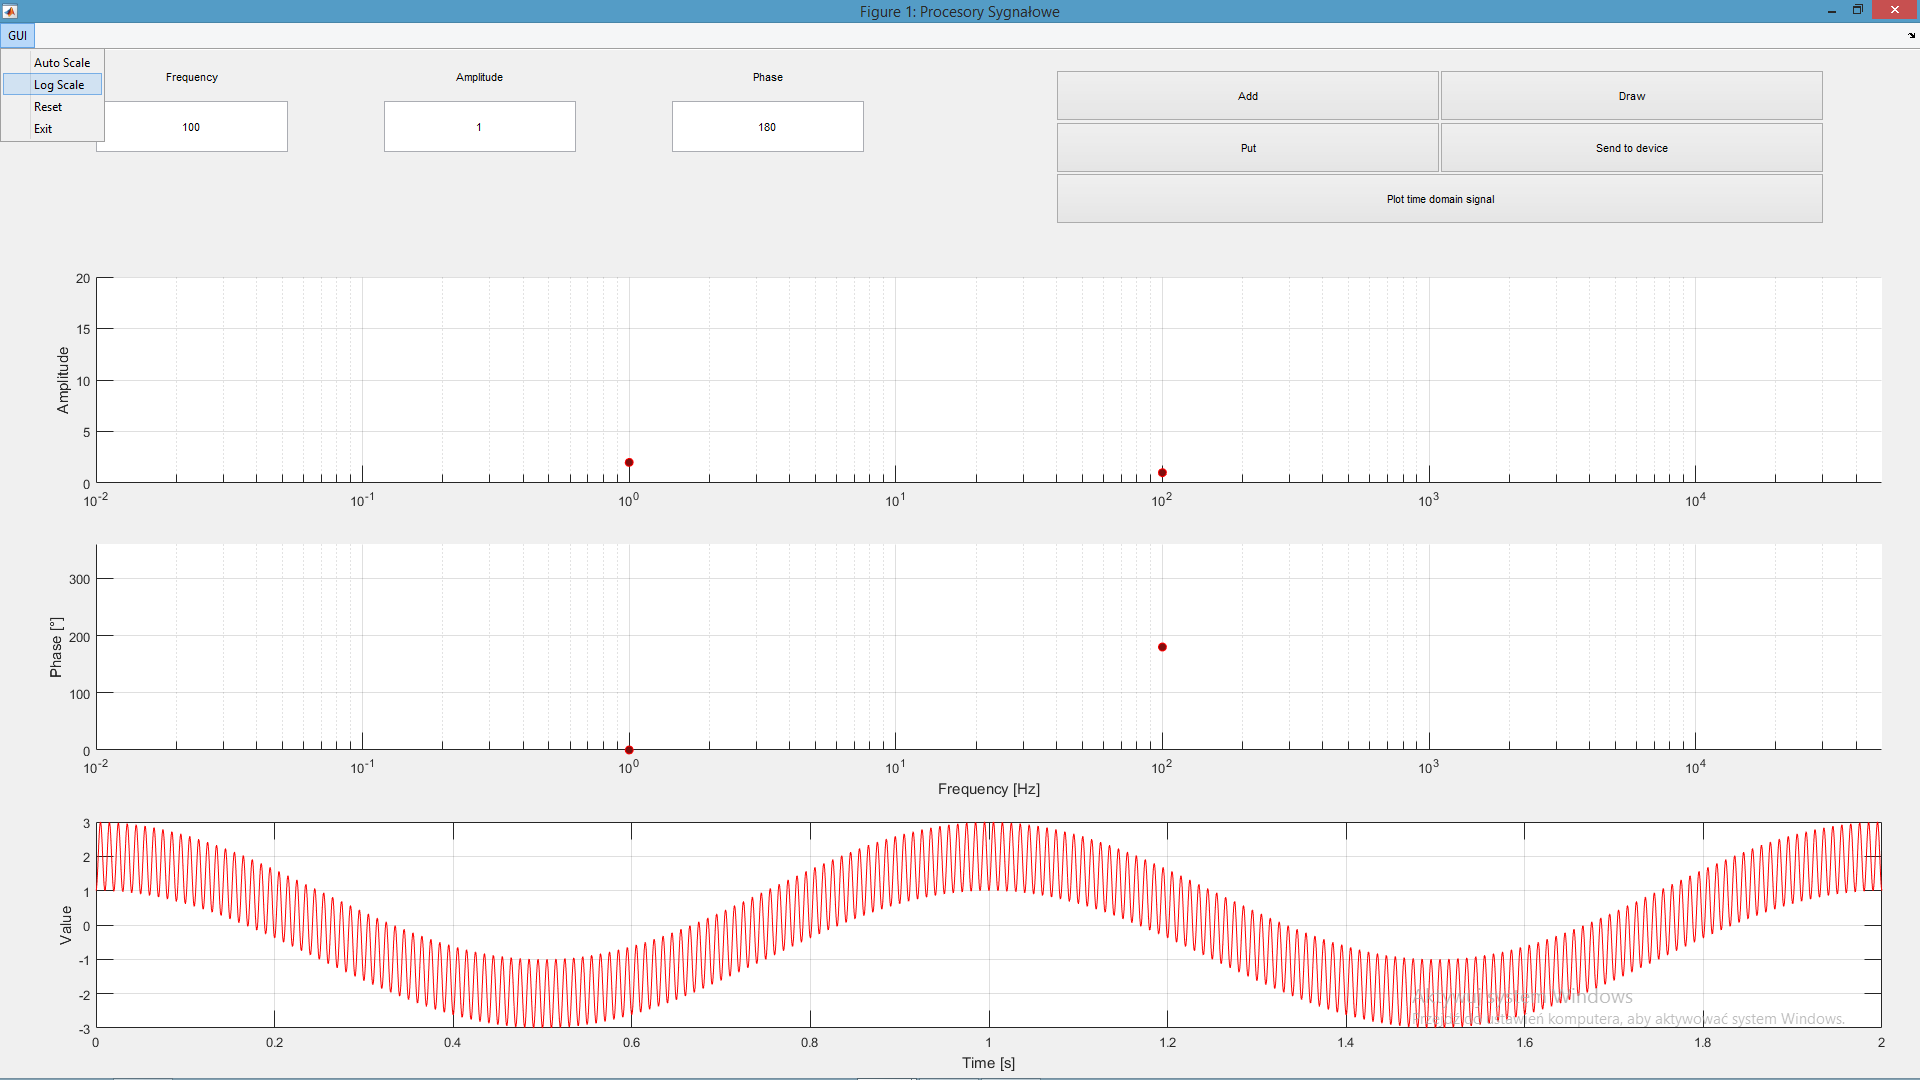
\includegraphics[scale = 0.3]{fig/ls.png}
	\caption		
	{Wyświetlenie wprowadzonej charakterystyki w skali logarytmicznej.}
	\label{log}
\end{figure}
\begin{figure}[h!]
	\centering
	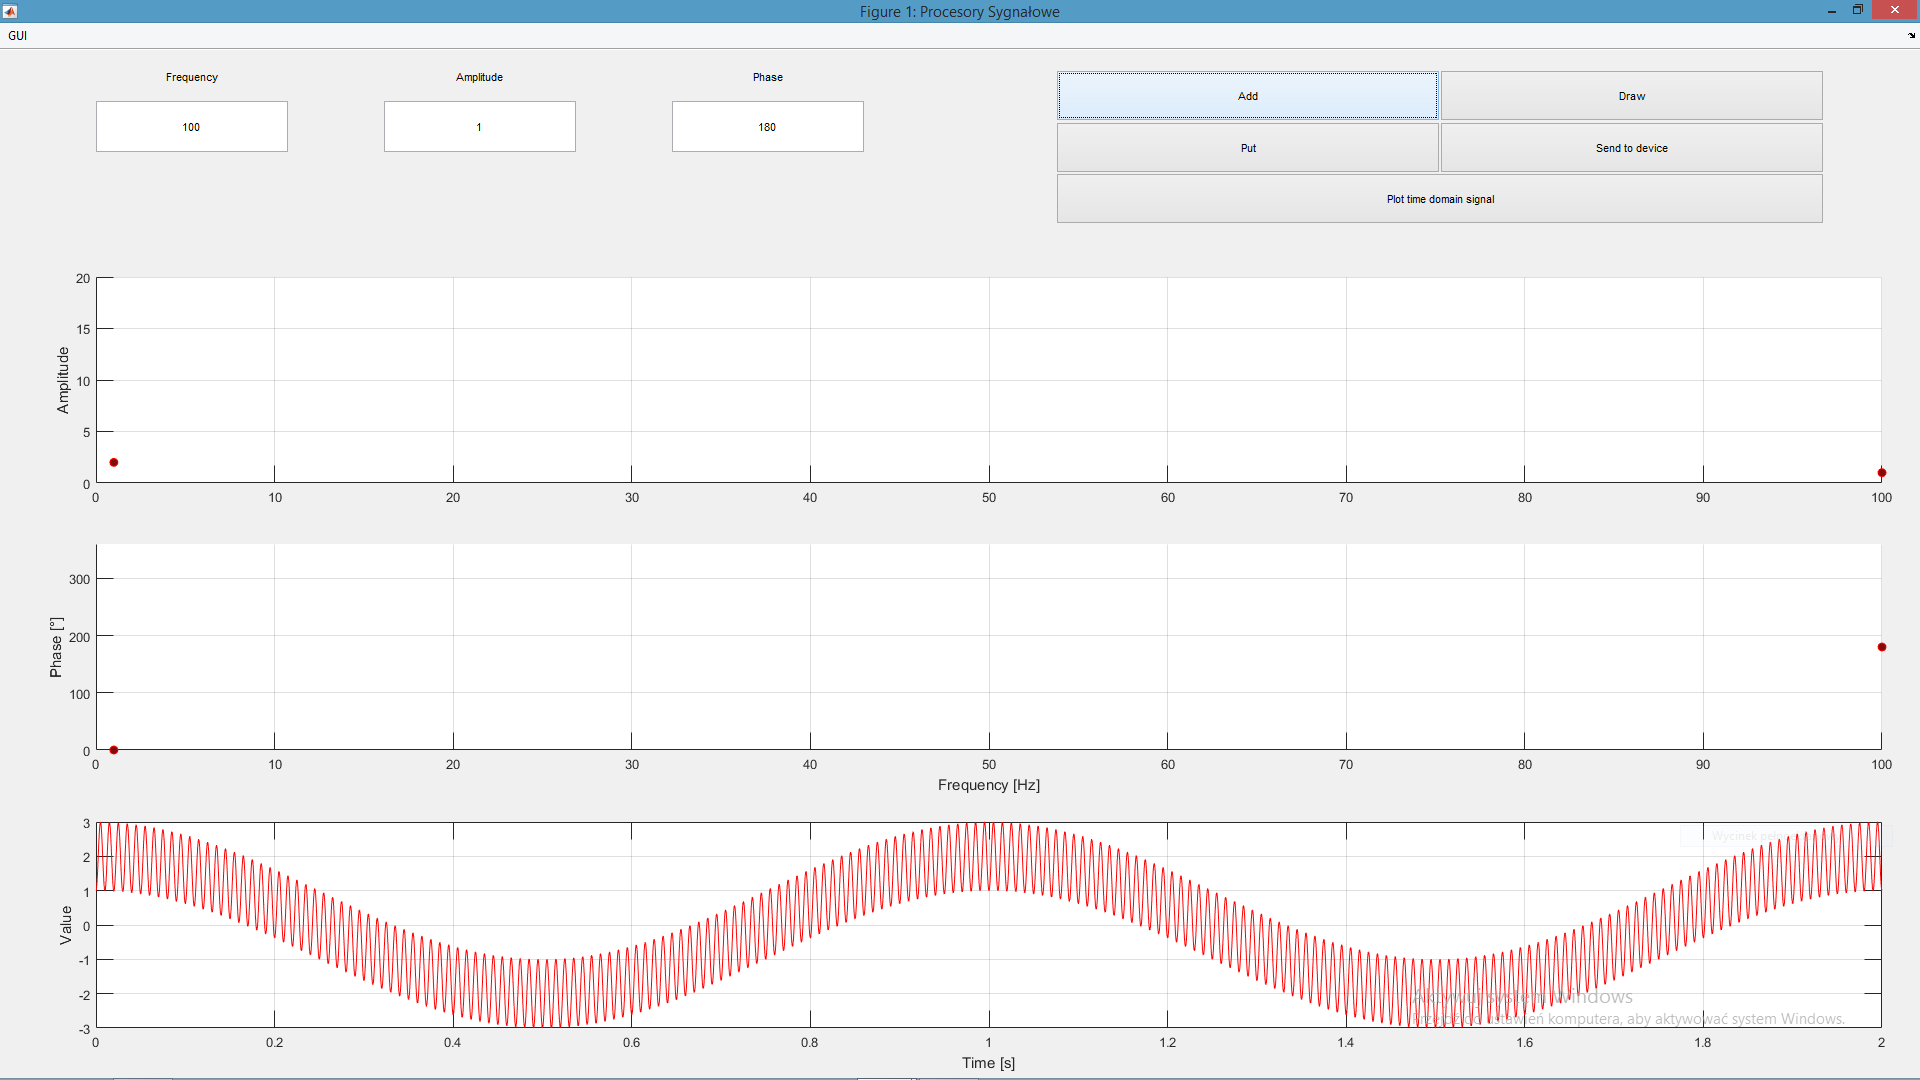
\includegraphics[scale = 0.3]{fig/as.png}
	\caption		
	{Wyświetlenie charakterystyki w skali liniowej - automatycznie dopasowanej do wprowadzonych punktów.}
	\label{as}
\end{figure}
W każdej chwili możliwe jest wygenerowanie wykresu w nowym oknie w sposób umożliwiający łatwy zapis, a także porównanie z sygnałem wyliczonym prze mikrokontroler. Po naciśnięciu przycisku \textit{Plot time domain signal} pojawi się wykres \ref{tds}.
\begin{figure}[h!]
	\centering
	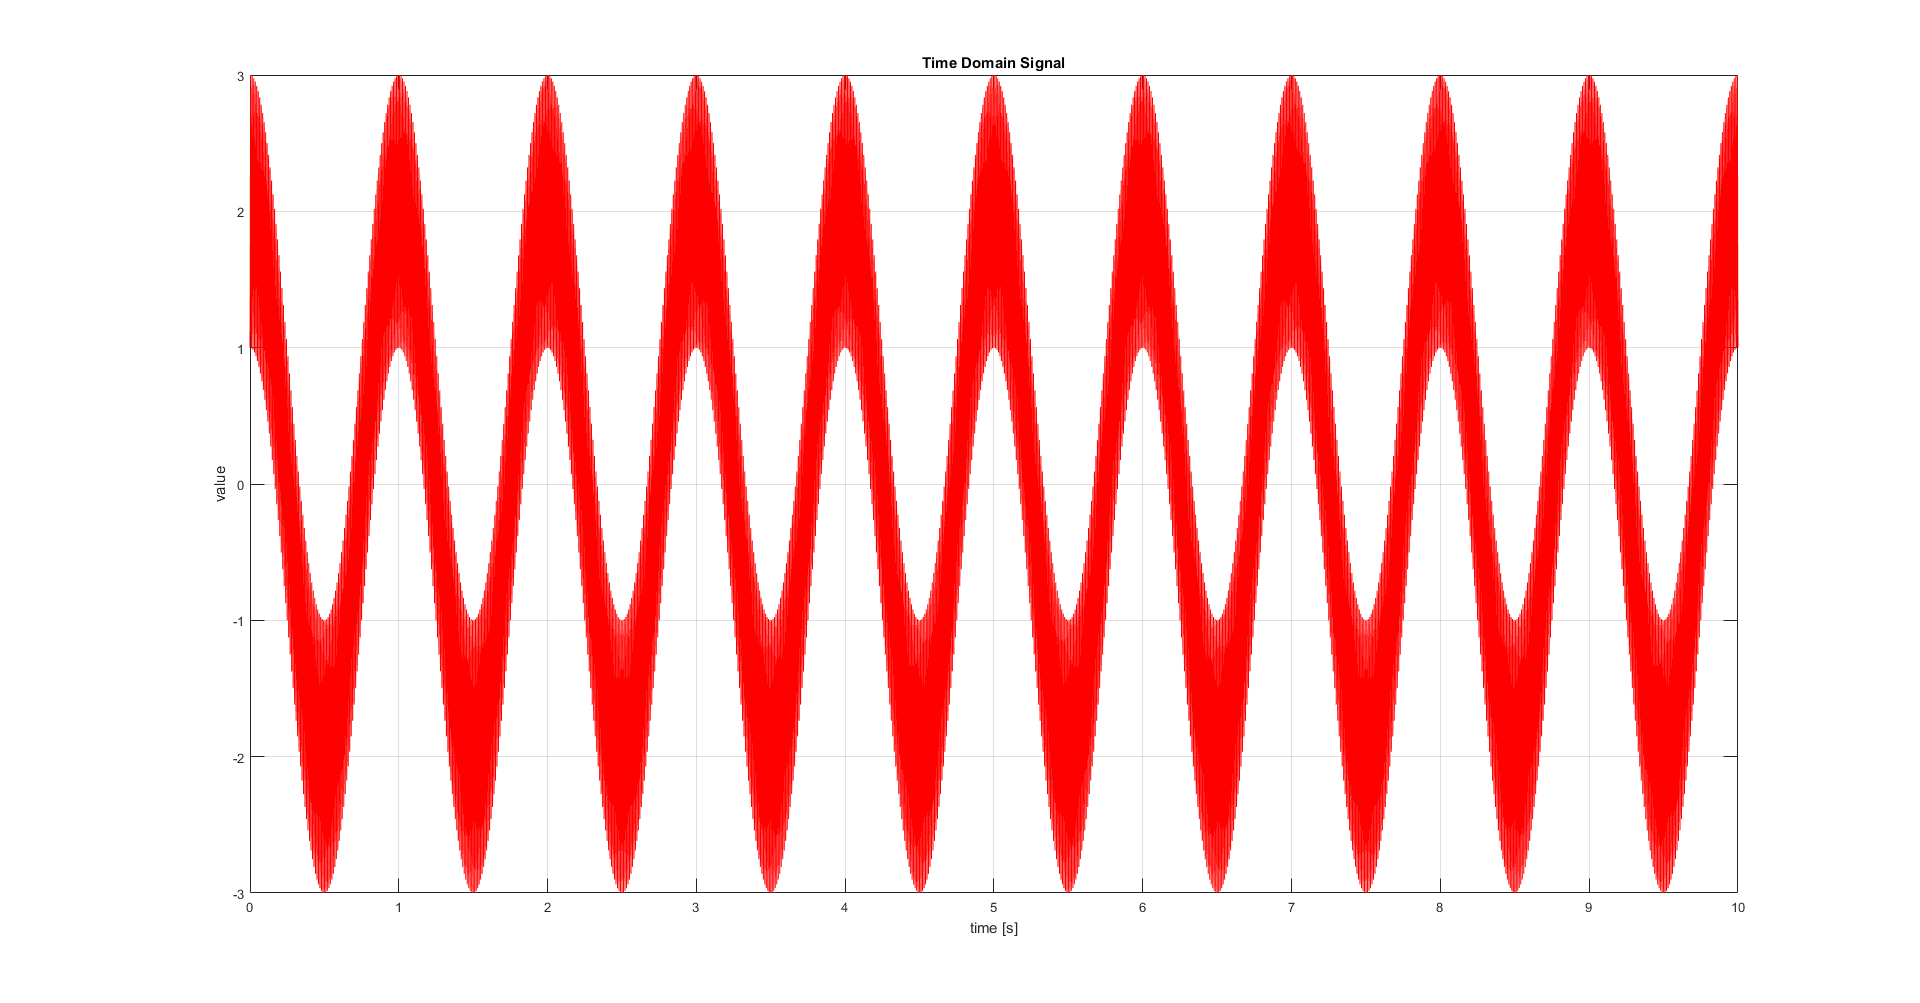
\includegraphics[scale = 0.3]{fig/tds.png}
	\caption		
	{Wykres w dziedzinie czasu.}
	\label{tds}
\end{figure}
Użytkownik po wciśnięciu przycisku \textit{Put} może ręcznie wprowadzić kolejny punkt charakterystyki poprzez najechanie kursorem w odpowiednie miejsce na wykresach - amplitudy oraz przesunięcia fazowego.
\begin{figure}[h!]
	\centering
	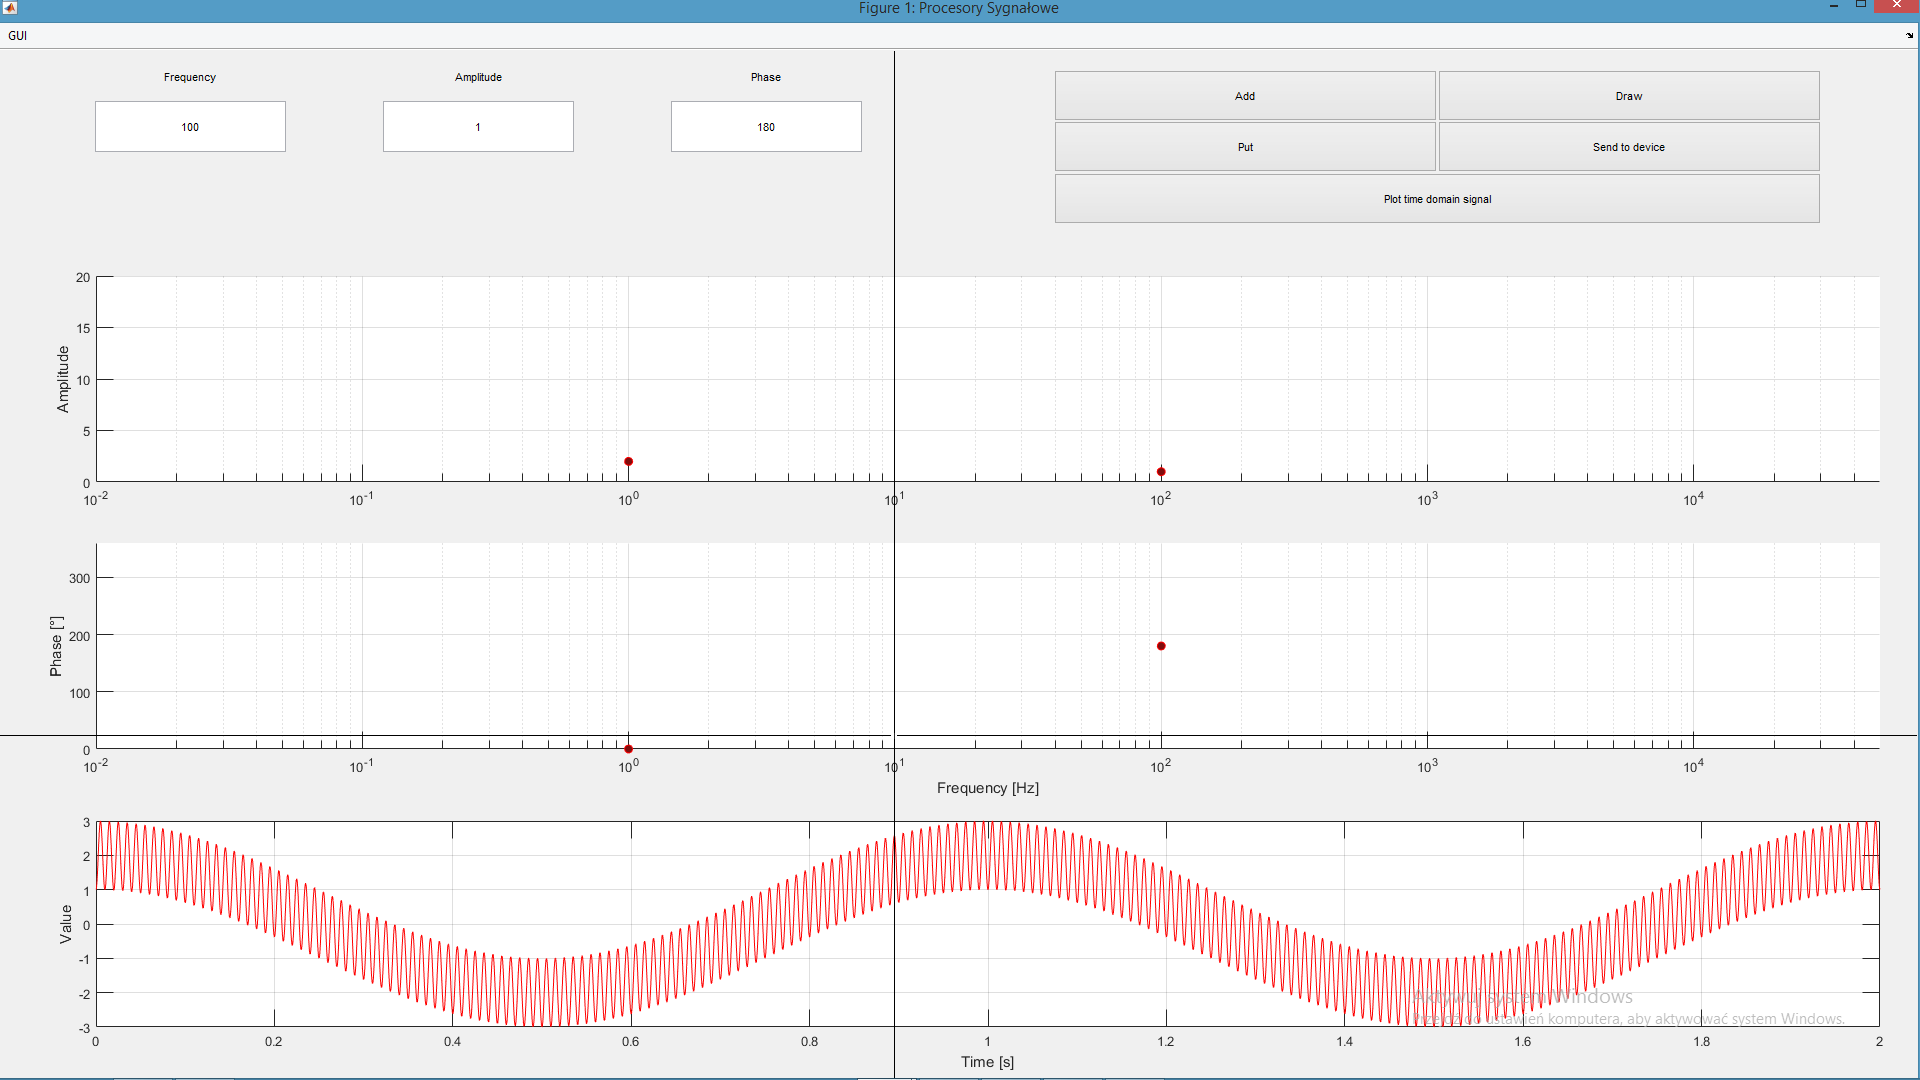
\includegraphics[scale = 0.3]{fig/put.png}
	\caption		
	{Wprowadzanie punktów do charakterystyki częstotliwościowej za pomocą kursora.}
	\label{fig:put}
\end{figure}
Po wciśnięciu lewego przycisku myszy w sytuacji zobrazowanej na rysunku \ref{fig:put} główny ekran aplikacji prezentuje się następująco - rys. \ref{fig:after}.
\begin{figure}[h!]
	\centering
	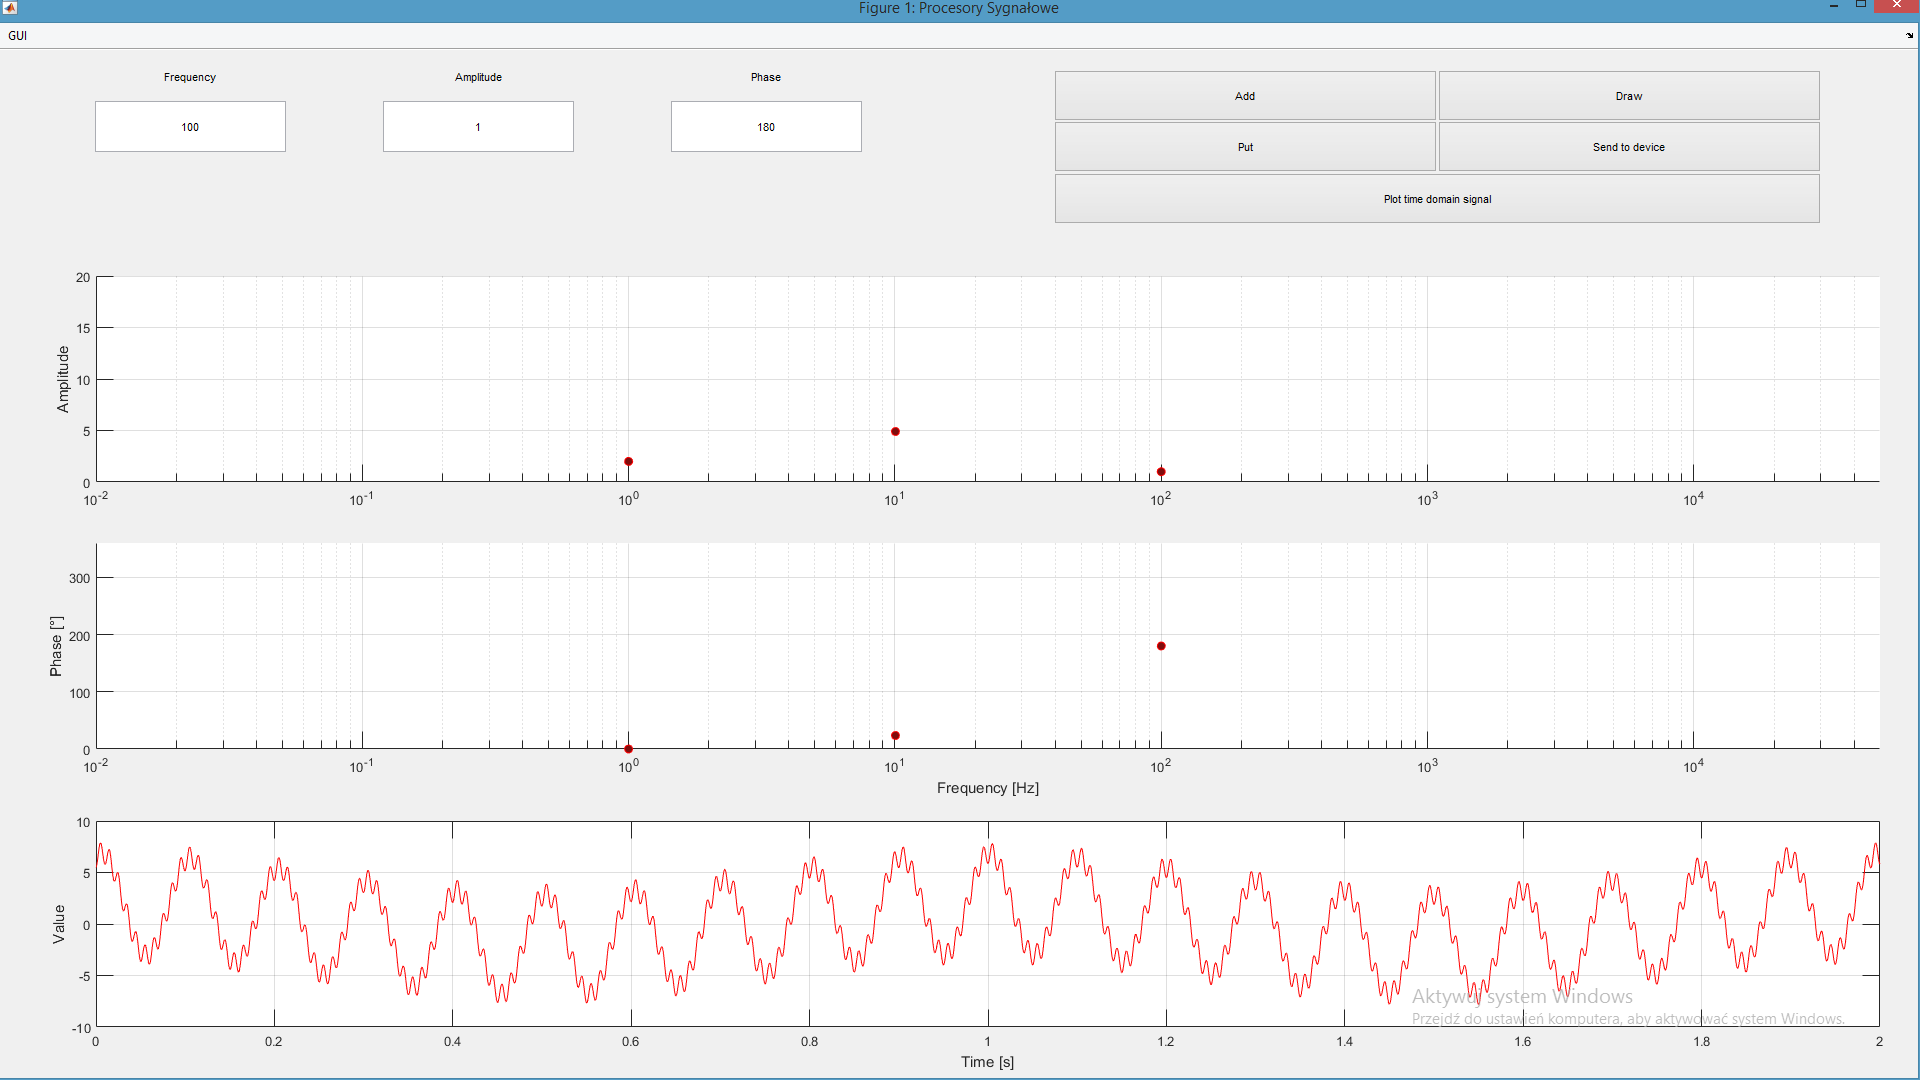
\includegraphics[scale = 0.3]{fig/after.png}
	\caption		
	{Ekran aplikacji po wprowadzeniu punktu za pomocą kursora.}
	\label{fig:after}
\end{figure}
\subsection{Protokół komunikacyjny}
\label{PK}
Dane z komputera do mikrokontrolera przesyłane są za pomocą protokołu \textit{RS232}, którego parametry podano w tabeli \ref{tab_rs232}. Specyfika implementowanego algorytmu wymagała zaproponowania jednolitego sposobu przesyłania danych opisujących zadaną charakterystykę. \\
Należało uwzględnić następujące czynniki:
\begin{enumerate}
	
	\item możliwość przesyłania dowolnie wielu zestawów danych opisujących pojedynczy punk charakterystyki, tzn. częstotliwość, amplitudę i przesunięcie fazowe,
	\item możliwość przesyłania nowego zestawu danych bez konieczności resetowania układu.
	\item liczy opisujące poszczególne współczynniki mogą mieć różną liczbę cyfr.
\end{enumerate}
%
%
Biorąc pod uwagę wszystkie powyższe wymagania oraz specyfikę protokołu \textit{RS232} zdecydowano się przesyłać dane w postaci pojedynczych znaków. Procedura \textit{składania} liczby z przesłanych znaków została zaimplementowana w samym urządzeniu. Aby algorytm mógł rozróżnić czy przesłany znak jest częścią obecnie składanej liczby czy dotyczy już następnego parametru, wprowadzono znak \textit{tabulacji}, który oddziela cyfry kolejnych liczb.
\\
Przyjęto, że pierwsza liczba przesłana do mikrokontrolera określa liczbę punktów charakterystyki. Następnie przesyłane są kolejne zestawy danych składające się z trzech liczb: częstotliwości, amplitudy i przesunięcia fazowego. Każda z tych trzech liczb zapisywana jest w odpowiedniej tablicy.
\\
Do przechowywania poszczególnych wartości wykorzystywane są dwa zestawy dynamicznie alokowanych tablic. Pierwszy zestaw służy do przechowywania danych obecnie generowanego sygnału, natomiast drugi wykorzystywany jest do zapisywania aktualnie przesyłanego zestawu. 
\\
Po przesłaniu wszystkich liczb pamięć przeznaczona na pierwszy zestaw tablic jest zwalniana. Do wska\'zników, które wcześniej przechowywały adresy pierwszego zestawu przepisywane są adresy zestawu drugiego. Dzięki operacjom na wska\'znikach zaoszczędzono czas potrzebny na przepisywanie danych z jednego zestawu do drugiego. 
\\
Kod od przerwania odebrania nowego znaku zamieszczony jest na listingu \ref{uart_rec}
\begin{lstlisting}[frame=single, caption = Implementacja protokołu komunikacji, label = uart_rec]
void HAL_UART_RxCpltCallback(UART_HandleTypeDef *huart) {

static int i=0;
static int sample_iter = -1;
static int liczbaProbek = -1;
static int idTab = 0;
uint8_t data[50];
uint16_t size = 0;

// procedura "skladania" liczby z przeslanych cyfr

if(Received == 9 || i==ReceivedTabSize) // zatwierdzenie liczby TABem
{
volatile uint8_t recNumber = 0;
for (int k=0;k<i;k++)
{
recNumber += power(i-k-1) * ReceivedTab[k];
}
i = 0;

//odebranie pierwzej liczby okreslajacej liczbe przesylanych 
//punktow
if(sample_iter == -1)
{
liczbaProbek = recNumber;
MAX = liczbaProbek;
freqTabRT = malloc(liczbaProbek*sizeof(uint8_t));
ampTabRT = malloc(liczbaProbek*sizeof(uint8_t));
phaseTabRT = malloc(liczbaProbek*sizeof(uint8_t));
sample_iter = 0;
}
else
{
size = sprintf(data, "echoProbki:\t %u \n\r", recNumber);
HAL_UART_Transmit_IT(&huart2, data, size);
if(sample_iter%3 == 0) // freq
{
freqTabRT[idTab] =  recNumber;
freq = recNumber;
}
else if(sample_iter%3 == 1) // amp
{
ampTabRT[idTab] = recNumber;
}
else if(sample_iter%3 == 2) // phase
{
phaseTabRT[idTab] = recNumber;
idTab++;
}
sample_iter += 1;
}
if(idTab == liczbaProbek)
{
free(freqTab);
free(ampTab);
free(phaseTab);
freqTab = freqTabRT;
ampTab = ampTabRT;
phaseTab = phaseTabRT;

size = sprintf(data, "koniec \n\r");
HAL_UART_Transmit_IT(&huart2, data, size);
sample_iter = -1;
idTab = 0;
}

}
else
{
ReceivedTab[i] = atoi(&Received);
i++;
}

// ponowne wlaczenie odbierania
HAL_UART_Receive_IT(&huart2, &Received, r_size);
}

int power(int a)
{
int wynik = 1;
for (int i=0;i<a;i++)
wynik *= 10;
return wynik;
}
\end{lstlisting}
\subsection{Generacja sygnału wyjściowego}

Sygnał wyjściowy generowany jest na podstawie algorytmu opisanego w rozdziale \ref{algorytm}, cyklicznie w przerwaniu od timera nr 11. Kod wyliczający odwrotną transformatę przedstawiony jest listingu \ref{fourierKod}. 
%
\begin{lstlisting}[frame=single, caption = Kod funkcji obliczającej odwrotną transformatę Fouriera w przerwaniu od timera 11., label = fourierKod]
void HAL_TIM_PeriodElapsedCallback(TIM_HandleTypeDef *htim)
{
	static long long int t = 0;
	int index = 0;
	
	float v;
	
	if(htim->Instance == TIM11){
	
		HAL_DAC_SetValue(&hdac,DAC_CHANNEL_1,DAC_ALIGN_12B_R,output);
		if(freqTab==NULL || ampTab==NULL ||phaseTab==NULL)
		{
			return;
		}
		out = 0;
		t=t+1;
		for (int ii=0;ii<MAX;ii++)
		{
			v = 360 * tp * freqTab[ii]*t + 180 - phaseTab[ii];
			cos = cosApproximation(v);
			out = out + ampTab[ii]*cos;
		}
		
		// skalowanie amplitudy -50 do 50 na od 0 do 4095
		output = (int)(out*40.96 + 2048);
	}
}
\end{lstlisting}
%
Aby zaoszczędzić czas potrzebny na wyliczanie wartości cosinusa kąta w każdej iteracji pętli algorytmu zdecydowano się na zapisanie wartości tej funkcji w pamięci mikokontrolera z rozdzielczością $1^0$. Rozdzielczość ta jest w wielu wypadkach zadawalająca, jednak w przypadkach wymagających większej precyzji można skorzystać z funkcji \mbox{\textit{cosApproximation}}, której kod podano w listingu \ref{cosApp}, a która to aproksymuje wartość cosinusa kąta funkcją liniową pomiędzy dwiema stablicowanymi wartościami. \\

\begin{lstlisting}[frame=single, caption = Funkcja aproksymująca wartość cosinusa., label = cosApp]
inline float cosApproximation(float v)
{
	float value = 0;
	
	uint16_t a = ((int) v) % 360;
	uint16_t b = (a + 1) % 360;
	
	float cos_a = cosTable[a];
	float cos_b = cosTable[b];
	wsp_a = cos_b - cos_a;
	wsp_b = cos_a - wsp_a * a;
	
	value = wsp_a * (v - (int)(v) + a) + wsp_b;
	
	return value;
}
\end{lstlisting}
